\section{Introduction}
\label{sec:intro}

\newcommand{\seedefs}{(formally defined in \ref{sec:appendix:defs})}
\newcommand{\seedefsb}{(see \ref{sec:appendix:defs} for definitions)}
\newcommand{\seedefsc}{See \ref{sec:appendix:defs} for formal definitions}
\newcommand{\seedefsd}{see \ref{sec:appendix:defs} for definitions}
\newcommand{\seedefsprelim}{(formally defined in Section \ref{sec:prelim:defs})}


% \todo{Regarding qusecs... We use the standard way of dealing w/ these problems, namely modeling it as a geometric constraint system...
% \todo{Restructure intro so that we have... problems first... closing with ``Concerning these issue... this is what we do in relation to them... the specifics we address..'' and go into summary of our contributions}

Geometric constraint systems have well-established, mature applications in mechanical engineering and  robotics, and they continue to find emerging applications in diverse fields from machine learning to molecular modeling.  Solving or realizing geometric constraint systems requires finding real solutions to a large multivariate polynomial system (of equalities and inequalities representing the constraints); this requires double exponential time in the number of variables, even if the type or orientation of the solution is specified.
% Thus, recursive decomposition into locally rigid subsystems (which have finitely many solutions) is crucial for realizing a geometric constraint system by the reverse process of recombining the subsystem solutions.
Thus, to realize a geometric constraint system, it is crucial to perform recursive decomposition into locally rigid subsystems (which have finitely many solutions), and then apply the reverse process of recombining the subsystem solutions.
With the use of \dfn{decomposition-recombination (DR-) planning}, the complexity is dominated by the size of the largest subsystem that is solved, or recombined, from the solutions of its child subsystems, i.e.\ the maximum fan-in occurring in a DR-plan.
In addition, navigating and analyzing the solution spaces, as well as designing constraint systems with desired solution spaces, leads to the \dfn{optimal decomposition-recombination (DR-) planning} problem~\cite{sitharam2005combinatorial, hoffman2001decompositionI, hoffman2001decompositionII}.

For a broad class of geometric constraint systems, local rigidity is characterized generically as a sparsity and tightness condition of the underlying constraint (hyper)graph~\cite{laman1970graphs,streinu2009sparse,tay1976rigidity,white1987algebraic}. This allows the generic DR-planning problem to be stated and treated as a combinatorial or (hyper)graph problem as we do in this paper.

Na{\"i}vely, the optimal DR-plan is used as follows. Each decomposed subsystem -- a node of the DR-plan -- is treated and solved as a polynomial system of constraints between its child subsystems. However, even in an optimal DR-plan, there can be arbitrarily many children at a node. In other words, even in the recursive decomposition given by an optimal DR-plan, the  size of the maximal indecomposable subsystem could be arbitrarily large.  It represents a bottleneck that dictates the complexity of solving or realizing the constraint system \cite{sitharam2010optimized,sitharam2006well,sitharam2010reconciling}.  We address this problem using the recently developed concept of \dfn{convex Cayley configuration spaces} \cite{sitharam2010convex,sitharam2011cayleyI,sitharam2011cayleyII,sitharam2014beast,sitharam2013caymos,wang2014cayley}. This allows for even greater reduction of the complexity by realizing large, indecomposable systems in a manner that avoids working with large systems of equations.
Specifically, we give an efficient technique for \dfn{optimally modifying} large indecomposable subsystems in a manner that reduces their complexity while preserving desired solutions; the modification ensures a convex Cayley configuration space, and the space can be efficiently searched to find a realization that satisfies the additional constraints of the original system.
This optimal modification  problem is a generalization of the previously studied problem of optimal completion of underconstrained systems \cite{sitharam2005combinatorial,joan-arinyo2003transforming}.

DR-plans are especially useful for constraint systems that exhibit some level of \dfn{self-similarity} and \dfn{quasi-uniformity}, in addition to isostaticity.  These properties can be leveraged to further reduce the complexity of both optimal DR-plan construction and recombination.
We consider 3 different types of constraint systems -- which we collectively call \dfn{qusecs} -- that are used to model, design, and analyze quasi-uniform or self-similar materials.
In the remainder of this section, we motivate the materials application and give the contributions and organization of the paper.

% In this paper, we introduce new techniques for the recursive decomposition and recombination of two dimensional independent (isostatic or underconstrained) constraint systems. The main contributions are a method to generate an optimal decomposition-recombination (DR-) plan
%  leveraging the quasi-uniformity and self-similarity present in many real world applications,
% Decomposition is crucial for realizing and designing the geometric constraint system and its properties such as rigidity, stability, and stress response to external loads. When realizing these sparsity-condition constraint systems, the task would require finding real solutions to a large multivariate polynomial system (of inequalities and equalities representing the constraints). Without decomposition to plan the recombination (DR-planning), this requires double exponential time in the number of variables (even if orientation type is specified). With DR-planning, the complexity is dominated by the size of the largest subsystem that is solved, or recombined from the solutions of its child subsystems, i.e., the maximum fan-in occurring in a DR-plan. Thus, finding an optimal DR-plan is important for realization.



% Without decomposition to plan the recombination (DR-planning), this requires double exponential time in the number of variables (even if orientation type is specified).




% \subsection{The Importance of an Optimal DR-plan}
% \subsection{Importance of an Optimal DR-plan}
% The use of a DR-plan in designing especially self-similar qusecs is immediately evident, shown in Figures \ref{fig:c2c3ofk33s} and \ref{fig:bodypindrp}.

% In fact, knowing an optimal DR-plan is crucial for design and analysis of even non-self-similar qusecs and their realizations with various desirable properties.


% Furthermore, recursive block decomposition of the rigidity matrix, stress space, and external stresses can be obtained using the DR-plan. Each block is the rigidity matrix of an isostatic subgraph. The blocks intersect on isostatic or trivial subgraphs. This recursive block decomposition of the rigidity matrix $R$ corresponds to a recursive decomposition of the stress vectors $s$ that balance a given external stress $t$ since $sR = t$. Moreover, the external stress vector $t$ is recursively ``distributed'' into external stresses for each node of the DR-plan. When the rigidity matrix and stress vectors contain indeterminates, this can be used to design underlying graph and parameters $\delta$ to obtain an optimal distribution of stresses on the geometric primitives. When the realization of the system \nameit is given, this can be used to analyze the distribution of a given external load.



%highly general geometric constraint systems with the  This characterization has broad applicability in practice, and we provide several concrete examples.



% In the literature, this problem is called the optimal decomposition recombination (DR-) planning problem, which,
%An optimal DR-plan decreases the computation involved in such tasks; however, in general, finding an optimal DR-plan is NP-hard. Therefore, previous algorithms for the problem did not consider optimality and instead focused on other desirable criteria of the output DR-plan.
% Knowing an optimal DR-plan is crucial when working with isostatic geometric constraint systems with an underlying sparsity condition \nameit. It allows for efficient design and analysis of these systems with various desirable properties. The importance of an optimal plan is particularly evident when these systems \nameit are self-similar or quasi-uniform, shown in Figures \ref{fig:c2c3ofk33s} and \ref{fig:bodypindrp}, as the complexity of the plan is even further reduced.




% Instead, we propose the modification of the subsystem to find a convex configuration space that can be efficiently searched for a solution to the original system.
%Instead, we make use of the notion of Cayley complexity to quantify the difficulty of each step of recombination.
% We additionally use the notion of Cayley complexity to quantify the difficulty of each step of recombination. Once a subsystem is found that has a convex Cayley configuration space, the space can be efficiently searched to find a realization that satisfies the additional constraints of the original system.
% This allows for even greater reduction of the complexity, by realizing large, indecomposable systems in a way that avoids working with large systems of equations.



\subsection{Introducing Qusecs}
A large class of constraint systems that we call \dfn{qusecs}, a contraction of ``quasi-uniform or self-similar constraint system'', (a) can be treated combinatorially as described above and (b) occur as independent (isostatic or underconstrained) systems in materials applications. We discuss these next.
%
Some natural and engineered materials can be analyzed by treating them as two dimensional (2D) layers. As illustrated by the examples below, the structure within each layer is often: self-similar\footnote{In this manuscript we only study finite 2D structures. \dfn{Self-similarity} refers to the result of finitely many levels of hierarchy or subdivision in an iterated scheme to generate self-similar structures.}~\cite{2012arXiv1204.6389G}, spanning multiple scales; generally aperiodic and quasi-uniform within any one scale; and composed of a few repeated motifs appearing in disordered arrangements.
Note that a 2D layer is not necessarily planar (genus 0), it can consist of multiple, inter-constraining planar monolayers. Furthermore, a layer is often  either \dfn{isostatic} or \dfn{underconstrained} (not \dfn{self-stressed}/\dfn{overconstrained}, \seedefsd). These properties, as well as quasi-uniformity, aperiodicity, self-similarity, and layered structure, are natural consequences of evolutionary pressures or design objectives such as stability, minimizing mass, optimally distributing external stresses, and participating in the assembly of diverse and multifunctional, larger structures.
%

The importance of an optimal DR-plan is particularly evident for a qusecs. The quasi-uniform or self-similar properties mean that the decomposition and solution for one subsystem can be used as the decomposition and solution for other subsystems, thus causing further reduction in the complexity of both DR-planning and recombination. This is shown in Figures \ref{fig:c2c3ofk33s} and \ref{fig:bodypindrp}.



% \FigInit{}{fig:material_examples}
% \FigThreeSubfig%
%   {../../img/Chlamydomonas_TEM_17}
%   {Cross section of the Chlamydomonas algae axoneme, a cilia composed of microtubules~\cite{wikimediacommons2007cilia}.}
%   {fig:material_examples:microtubule}%
%   %
%   {../../img/ligten2}
%   {Cross section of a tendon displaying the hierarchical structure~\cite{lecture_biosolid_mechanics}.}
%   {fig:material_examples:tendon}%
%   %
%   {../../img/Rothemund-DNA-SierpinskiGasket}
%   {A DNA array exhibiting the Sierpinski triangle~\cite{wikimediacommons2007dna}.}
%   {fig:material_examples:sierpinski}

\ClearMyMinHeight
\SetMyMinHeight{.32}{../../img/Chlamydomonas_TEM_17}
\SetMyMinHeight{.32}{../../img/ligten2}
\SetMyMinHeight{.32}{../../img/Rothemund-DNA-SierpinskiGasket}

\begin{figure*}\centering%
  %
  \begin{subfigure}{0.32\linewidth}\centering
    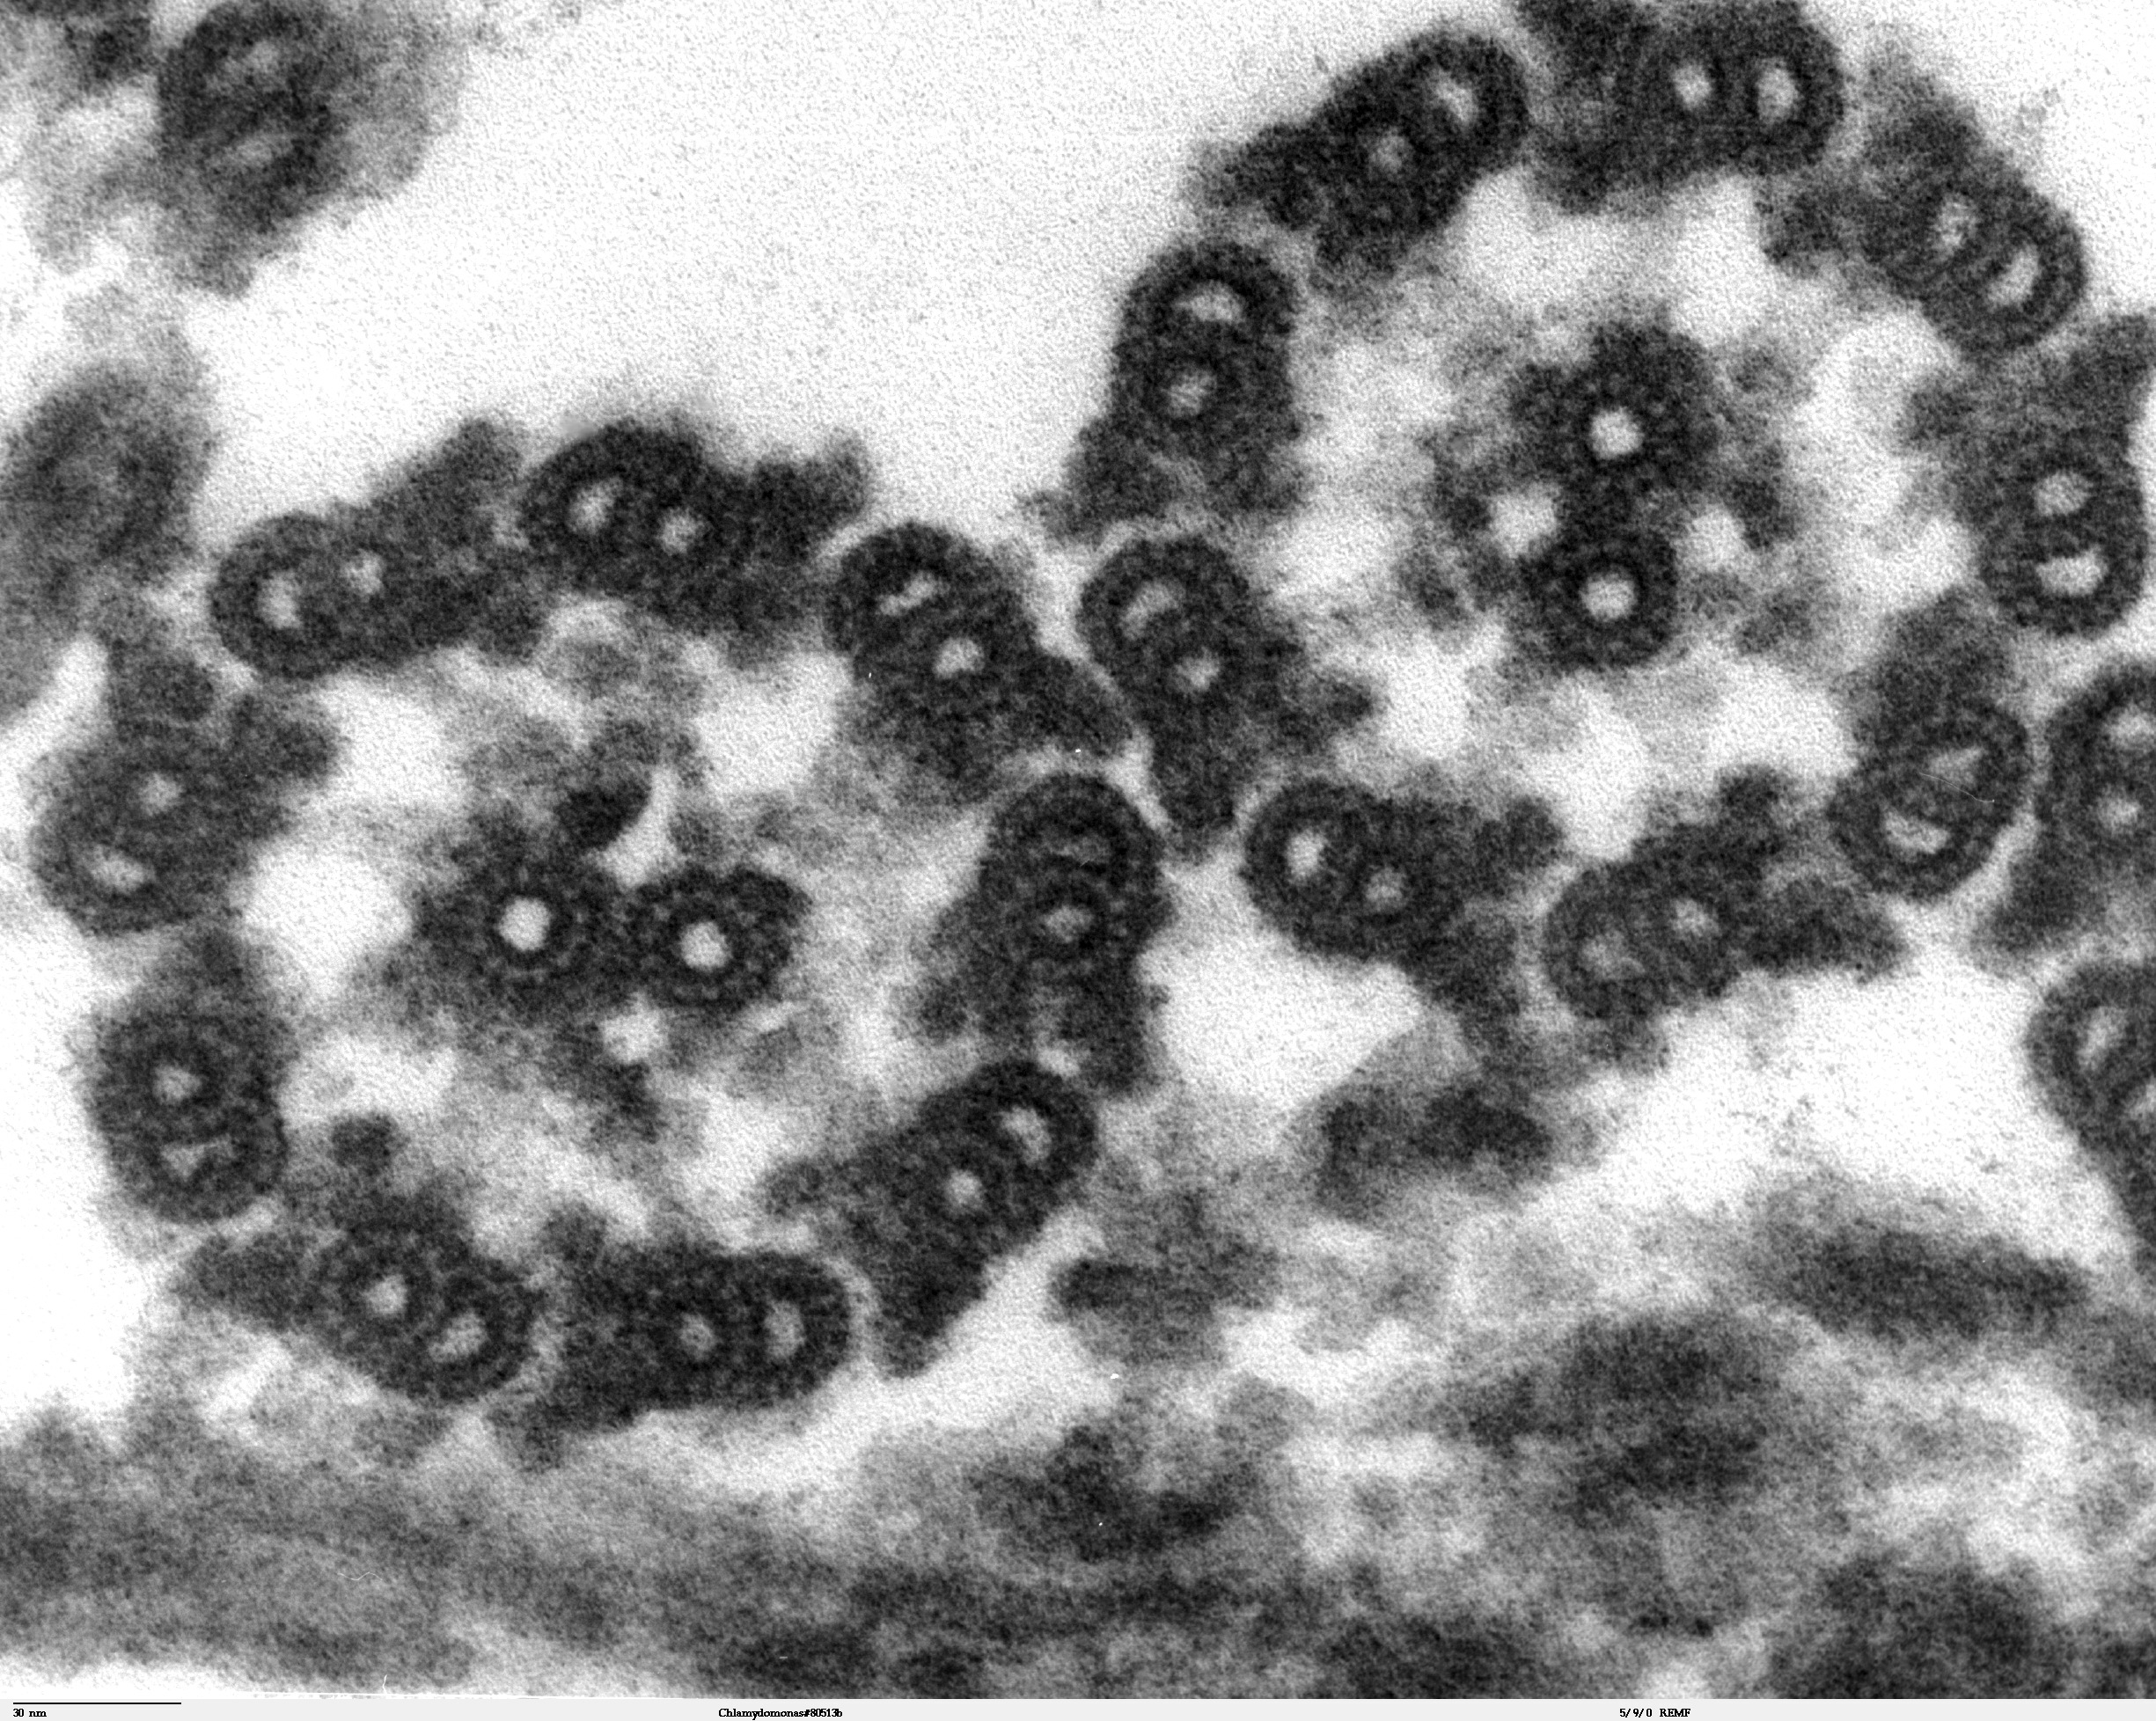
\includegraphics[height=\myMinHeight]{../../img/Chlamydomonas_TEM_17}
    \caption{}\label{fig:material_examples:microtubule}
  \end{subfigure}%
  %
  \hfill
  \begin{subfigure}{0.32\linewidth}\centering
    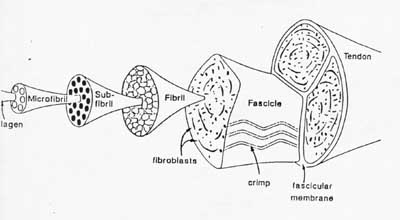
\includegraphics[height=\myMinHeight]{../../img/ligten2}
    \caption{}\label{fig:material_examples:tendon}
  \end{subfigure}%
  %
  \hfill
  \begin{subfigure}{0.32\linewidth}\centering
    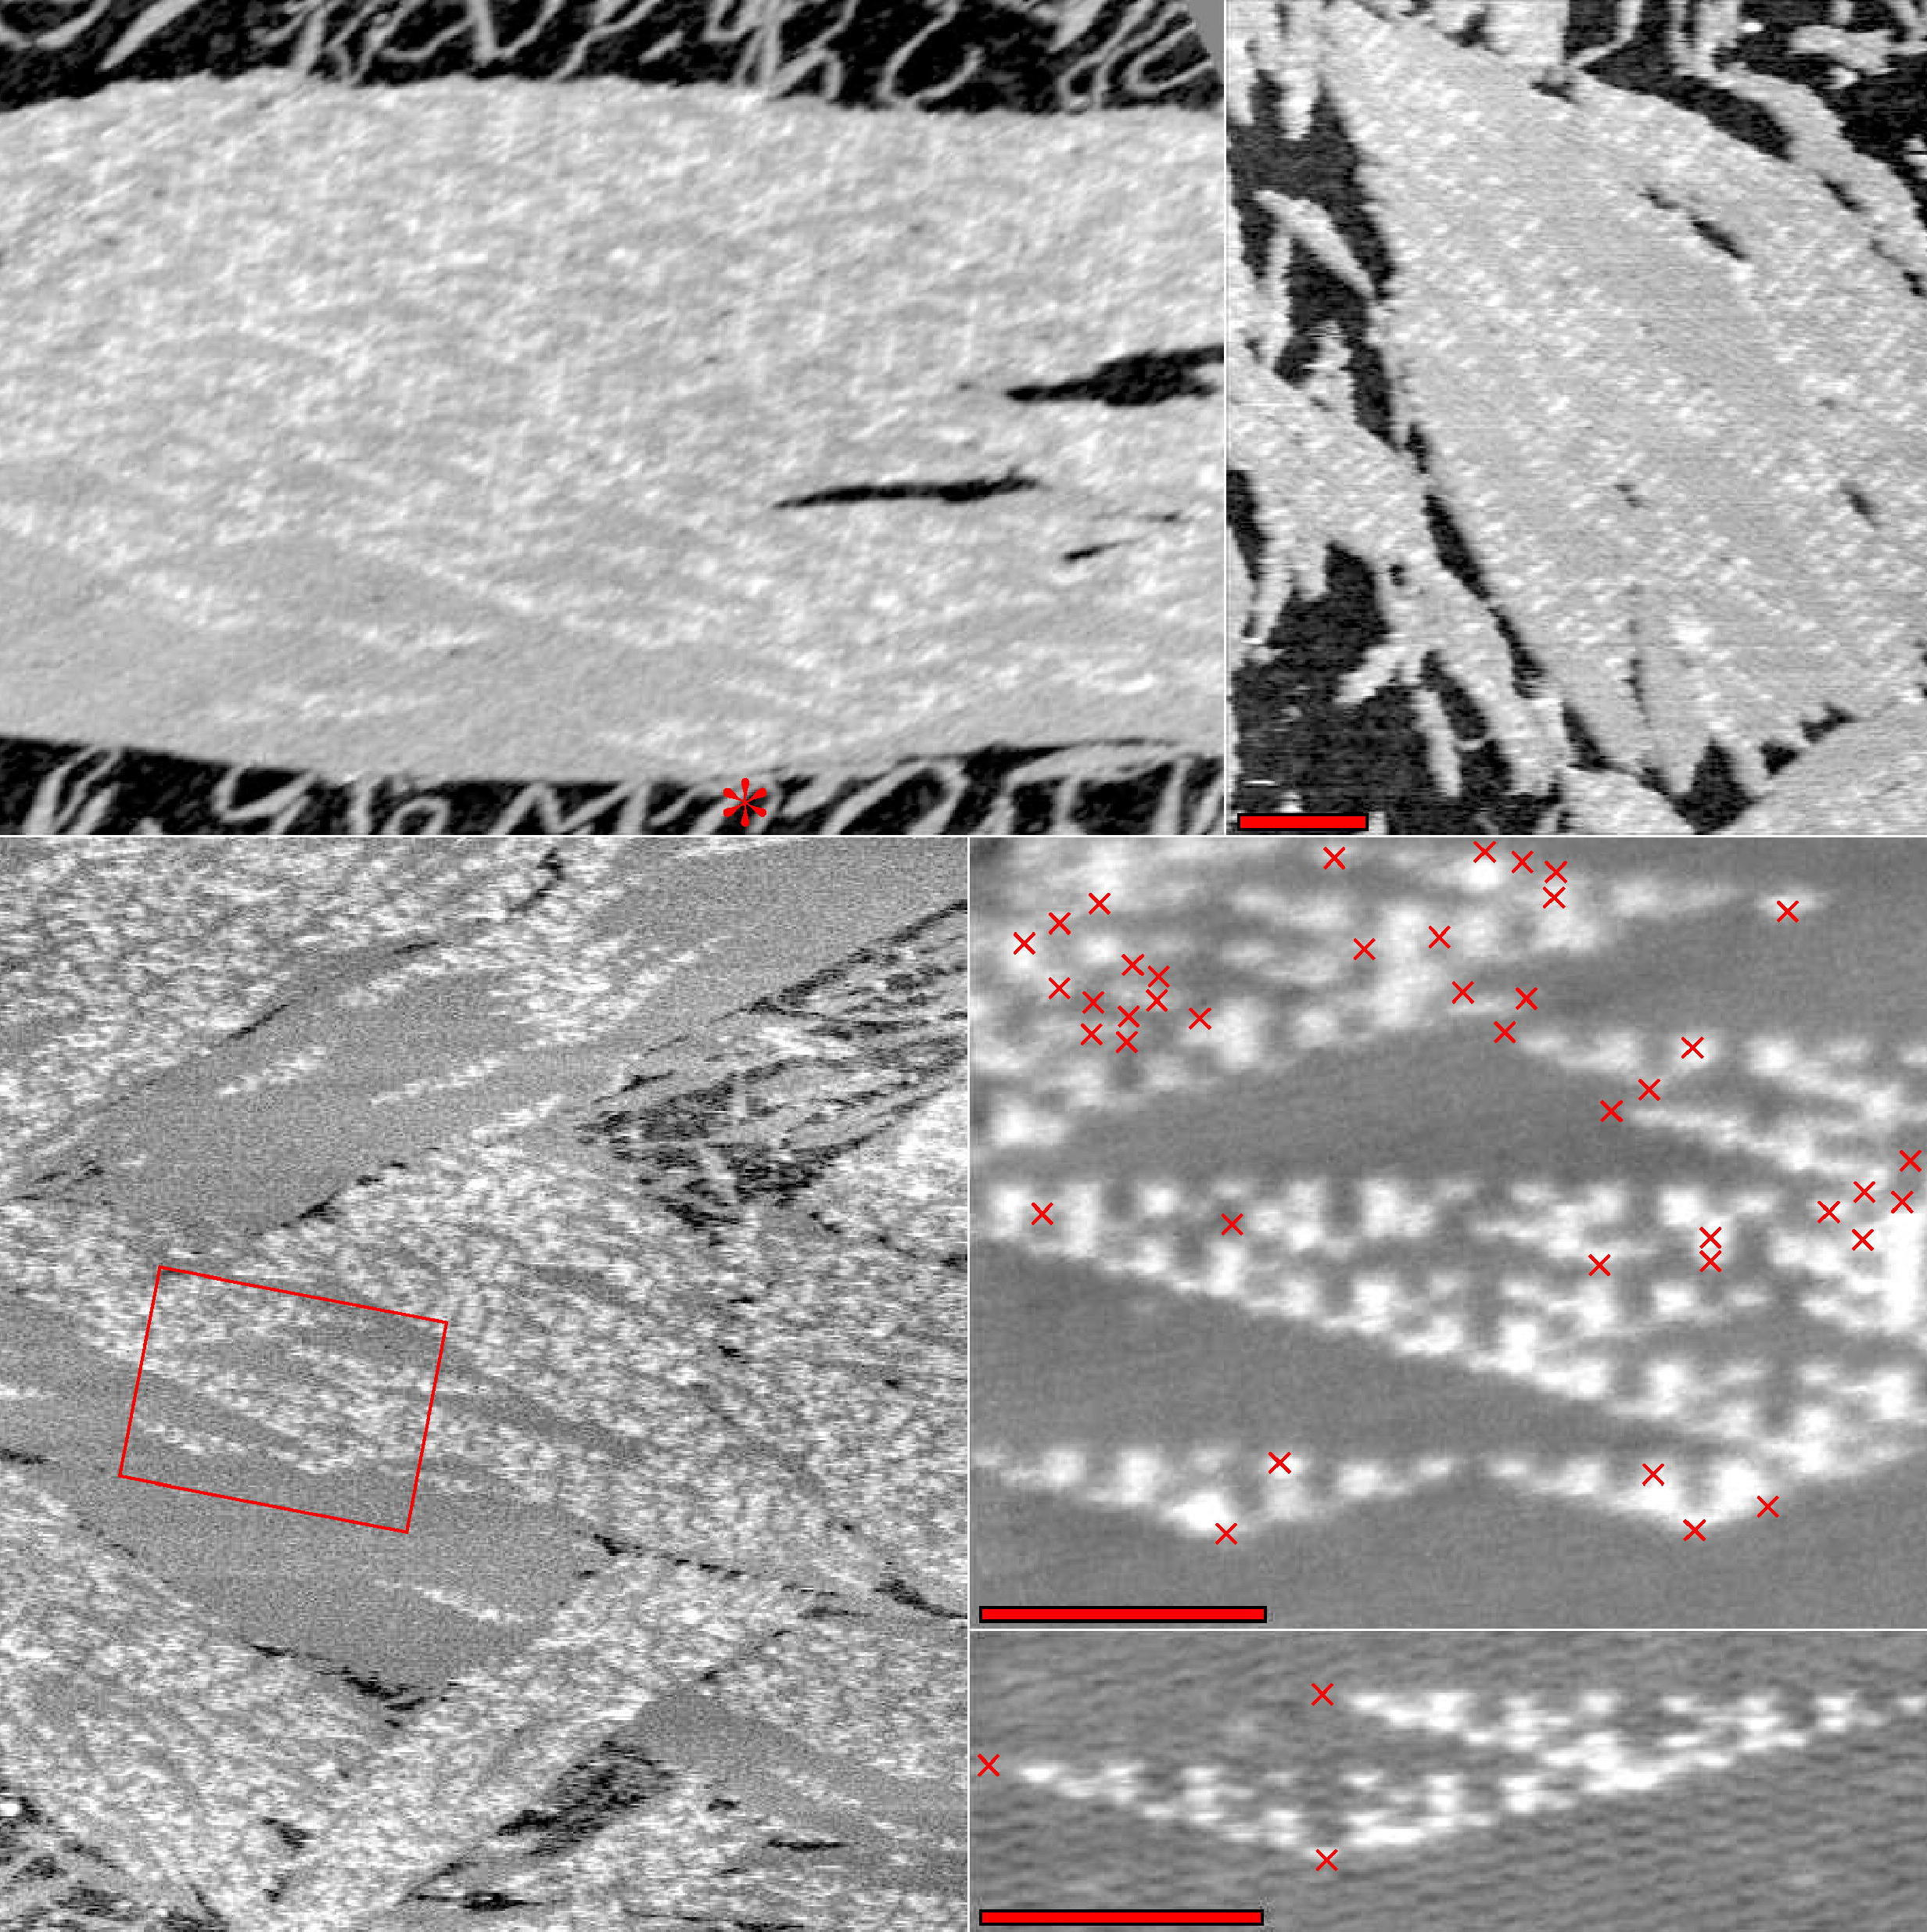
\includegraphics[height=\myMinHeight]{../../img/Rothemund-DNA-SierpinskiGasket}
    \caption{}\label{fig:material_examples:sierpinski}
  \end{subfigure}%
  %
  \caption{(\ref{fig:material_examples:microtubule}) Cross section of the Chlamydomonas algae axoneme, a cilia composed of microtubules~\cite{wikimediacommons2007cilia}. (\ref{fig:material_examples:tendon}) Cross section of a tendon displaying the hierarchical structure~\cite{lecture_biosolid_mechanics}. (\ref{fig:material_examples:sierpinski}) A DNA array exhibiting the Sierpinski triangle~\cite{wikimediacommons2007dna}.}\label{fig:material_examples}
\end{figure*}%


% \FigAddSubfig%
%   {0.3}
%   {../../img/Chlamydomonas_TEM_17}
%   {Cross section of the Chlamydomonas algae axoneme, a cilia composed of microtubules~\cite{wikimediacommons2007cilia}.}
%   {fig:material_examples:microtubule}%
% \FigAddSubfig%
%   {0.3}
%   {../../img/ligten2}
%   {Cross section of a tendon displaying the hierarchical structure~\cite{lecture_biosolid_mechanics}.}
%   {fig:material_examples:tendon}%
% \FigAddSubfig%
%   {0.3}
%   {../../img/Rothemund-DNA-SierpinskiGasket}
%   {A DNA array exhibiting the Sierpinski triangle~\cite{wikimediacommons2007dna}.}
%   {fig:material_examples:sierpinski}
% \FigDisplay{}{fig:material_examples}


% Examples of such materials (See Figure \ref{fig:material_examples}) include:
% In order to study structural and mechanical properties of a material layer, it is natural to model a material layer as a solution or realization of a geometric constraint system of appropriate types of geometric primitives, under metric or algebraic constraints.
% Such 2D \dfn{qusecs}, quasi-uniform or self-similar constraint systems \seedefsprelim, can be used to understand or design material layers (their solutions) with desired properties.
Some materials that are readily modeled as qusecs include:
%
\begin{enumerate}
    \item \label{materialexample1} Cross-sections of microtubule structures~\cite{microtubule_necklace} (Figure \ref{fig:material_examples:microtubule}), e.g., in ciliary membranes and transitions~\cite{microtubule_cilia}.

    \item \label{materialexample2} Cross-sections of organic tissue with hierarchical structure, e.g., compact bone and tendon (Figure \ref{fig:material_examples:tendon}).

    \item \label{materialexample3} Crosslinked cellulose or collagen microfibril monolayers, e.g., in cell-walls~\cite{wikimediacommons2010afm, wikimediacommons2007plant}, as well as crosslinked actin filaments in the cytoskeleton matrix. See Section \ref{sec:pinnedline}.

    \item \label{materialexample4} More recent, engineered examples, including disordered graphene layers~\cite{Graphene1, Graphene2} sometimes reinforced by microfibrils; and DNA assemblies including a recent Sierpinski gasket~\cite{self_assembly_sierpinski} (Figure \ref{fig:material_examples:sierpinski}), bringing other self-similar structures~\cite{wikimediacommons2012subdivision} within reach.

    \item \label{materialexample5} Silica bi-layers~\cite{silica_bilayers}, glass~\cite{sructure_of_2d_glass}, and materials that behave like assemblies of 2D particles under non-overlap constraints, i.e.\ like jammed disks on the plane~\cite{jammed_disks}. See Section \ref{sec:bodypin}.
\end{enumerate}




\subsection{Organization and Contributions}
\label{sec:cont}

In Section \ref{sec:prelim}, we provide basic definitions in combinatorial rigidity theory,  and formalize the new notion of qusecs~\cite{sitharam2010optimized,sitharam2006well,sitharam2010reconciling}.
In addition, we define DR-plans and what it means for a DR-plan to be complete or optimal. We survey previous work on DR-planning algorithms, discussing other desirable criteria of DR-plans and their relation to the NP-hard optimality property of DR-plans.
%This section is relevant to Examples \ref{materialexample1} and \ref{materialexample2},  model them as bar-joint systems and discuss achieving isostaticity, distribution of stresses in self-similar, and other important concepts. \todo{We don't model them as bar-joint... What did this mean originally?}

% In Section \ref{sec:DRP}, we navigate the NP-hardness barrier (discussed in the following subsection), for finding optimal DR-plans by defining a so-called \dfn{canonical} DR-plan and showing a strong Church-Rosser property: \vemph{all canonical DR-plans for isostatic or underconstrained 2D qusecs are optimal}.

% Also in Section \ref{sec:DRP}, we give an efficient (\ComplexityCanDRP) algorithm to find a canonical (and hence optimal) DR-plan for all 3 types of 2D qusecs mentioned above (Sections \ref{sec:DRP}, \ref{sec:bodypin}, and \ref{sec:pinnedline}).
% The canonical DR-plan elucidates the essence of the NP-hardness of finding optimal DR-plans for over-constrained systems.
% Furthermore, our optimal/canonical DR-plan satisfies desirable properties such as the previously studied Cluster Minimality \cite{hoffman2001decompositionI} (see Figure~\ref{fig:demo_graph:clustmindrp}).

In Section \ref{sec:DRP}, we define a so-called \dfn{canonical DR-plan} and prove a strong Church-Rosser property: all canonical DR-plans for isostatic or underconstrained qusecs are optimal. In so doing, we navigate the NP-hardness barrier present in the general form of the DR-planning problem; the canonical DR-plan elucidates the essence of the NP-hardness of finding optimal DR-plans when a system is over-constrained. Furthermore, our optimal/canonical DR-plan satisfies desirable properties such as the previously studied \dfn{cluster minimality}~\cite{hoffman2001decompositionI}. Also in this section, an \ComplexityCanDRP\ time algorithm is provided to find an optimal DR-plan for independent bar-joint graphs. While this and the next section focus on bar-joint graphs, the theory is easily extended to other qusecs used to model the abovementioned types of materials, as shown in subsequent sections.
% that such a plan will be optimal, in the sense that it minimizes the fan-in over all nodes, for isostatic bar-joint graphs.
% Additionally, a polynomial time (\ComplexityCanDRP) algorithm is provided to find a canonical DR-plan for isostatic bar-joint graphs.


In Section \ref{sec:recomb}, we give a method to deal with the algebraic complexity of recombining the realizations or solutions of child subsystems into a solution of the parent system \cite{sitharam2010optimized,sitharam2006well,sitharam2010reconciling}. Specifically, we define the problem of minimally modifying the indecomposable recombination system so that it becomes decomposable via a small DR-plan and yet preserves the original solutions in an efficiently searchable manner.
%
When the modifications are bounded, we obtain new, efficient algorithms for realizing both isostatic and underconstrained qusecs by leveraging recent results about Cayley parameters in \cite{sitharam2010convex,sitharam2011cayleyI,sitharam2011cayleyII} (see Sections \ref{sec:2-tree-reduction} and \ref{sec:tdecomp}).
%
In Section \ref{sec:table}, we show formal connection to well known problems such as optimal completion of underconstrained systems \cite{joan-arinyo2003transforming,sitharam2005combinatorial,gao2006ctree} and to find paths within the connected components.

% \todo{Section \ref{sec:recomb} addresses the issue of large, indecomposable subgraphs in the optimal DR-plan of bar-joint graphs by proposing a novel method of modification. By dropping edges to get a convex configuration space, realizations of the original linkage can be found. Also problem relations...}

 % The next sections focus on explicit applications by modeling certain materials as qusecs.

In Section~\ref{sec:bodypin} and~\ref{sec:pinnedline}, we briefly describe applications of the above techniques to modeling, analyzing, and designing specific properties in 2D material layers~\cite{Jackson2008bodypin}. We explicitly model these materials as qusecs. For Examples~\ref{materialexample4} and~\ref{materialexample5}, we discuss boundary conditions for achieving various desired properties of body-hyperpin systems. For Example~\ref{materialexample3}, we discuss canonical and optimal DR-plans for pinned line incidence systems~\cite{sitharam2014incidence}.

The last Section~\ref{sec:probs_and_conclusion} concludes the paper, and Section \ref{sec:open} lists open problems and conjectures. In particular, we conjecture that the methods of Section~\ref{sec:DRP} extend in fact to a large class of (hyper)graphs, formally those with an underlying abstract rigidity matroid in which independence corresponds to some type of sparsity, and maximal independence (rigidity) is a tightness condition.

Throughout this paper,  an asterisk after a formal statement indicates that its proof appears in~\ref{sec:appendix:proofs}.


A software implementation of our algorithms and videos demonstrating the software are publicly available online\footnote{See footnote 1.}.
